% !TEX root = ../TechProject.tex

\graphicspath{{Chapter6/}}

\chapter{Results and Discussion}

This chapter provides an analysis and discussion of the results from the experiment described
in Chapter 6. The experiment sought to answer the question presented in Chapter 5.
\\
\\
\textit{Is the proposed method a suitable solution to automate recommendations of songs suitable for adding to a given DJ set?}.
\\

Chapter 7.1 will present the appropriate latent factors to use on the dataset. Chapter 7.2 explores whether varying the DJ set size could improve the model's r-precision value.

\section{Latent Factors}
The controlled variable is the list of input DJ sets, and the independent variable is the number of latent factors for the alternating least squares part of the model. In the medium article, Chow used 50 latent factors \citep{chow_music_2020}. This was used as a reference point to make the range from 20 - 110 latent factors to experiment on. R-precision is the dependent variable.

Figure 7.1 shows a scatter graph of the average R-precision over different latent factors. The analysis shows that the application's performance varies significantly with the number of latent factors used. For example, the highest average r-precision of 0.1207 was obtained when 80 latent factors were used, while the lowest value of 0.0774 was obtained when only 20 latent factors were used. However, the algorithm's performance was not monotonically increasing or decreasing with the number of latent factors. For instance, there was a slight increase in average r-precision from 40 to 70 latent factors but a decrease from 50 to 60 latent factors. From 90 to 100, we see a significant decrease in the average r-value, which suggests that over-fitting is occurring.

\begin{figure}[H]
	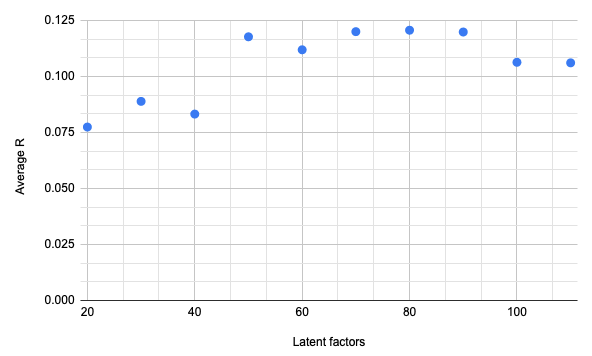
\includegraphics[scale=0.6]{images/average_r_over_latent}
	\centering
	\caption{Scatter graph of average r-precision values with different latent factors} 
\end{figure}

It is evident that too few and too many latent factors affect the model's performance. Therefore, balancing the number of latent factors and the algorithm's performance is vital.

\section{Varying input set length}
Given that an optimal latent factor value of 80 was determined, it is worth seeing if r-precision changes with the number of input songs in a DJ set. Increasing the input set size could improve the model's accuracy due to having more missing songs to pick from. The independent variable in this section is the evaluation set parameters, and the dependent variable is the average r-precision value.

In Figure 7	.2, a scatter graph illustrates the r-precision values of each DJ set when the number of latent factors was set to 80. The graph reveals that most sets scored zero, indicating that the recommendation system did not perform well for these sets. The highest score observed was 0.8, which suggests that the system provided a reasonably accurate recommendation for that particular set.

However, as the number of input songs in the DJ sets increased beyond 30, relatively fewer results were available, but none of the DJ sets had an r-precision value of zero. This finding suggests that the recommendation system improved its ability to provide accurate recommendations for sets with a larger number of input songs.

\begin{figure}[H]
	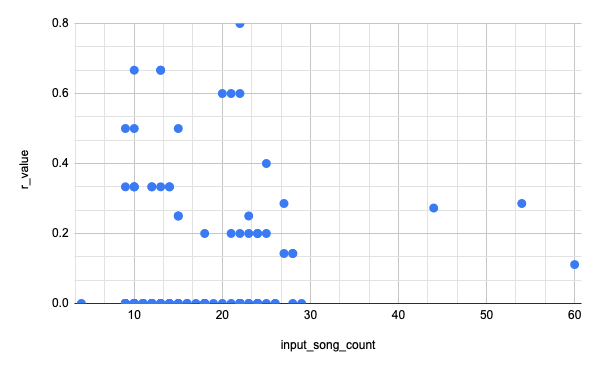
\includegraphics[scale=0.6]{images/80_little_sets}
	\centering
	\caption{Scatter graph of r-precision values with latent factors as 80} 
\end{figure}


When observing the changes in latent factors, the evaluation set was pulled from DJ sets that had 10 songs or more and included sets where each song had a total play count greater than 5. To focus on larger DJ sets, the total play count was lowered to 2 and then filtered on just DJ sets with over 20 songs.

Figure 7.3 shows the impact of input set size change on r-precision values, still using a latent factor value of 80. The results reveal that most DJ sets still had an r-precision value of zero. The highest r-precision value observed in this scenario was 0.6, and the average r-precision value was measured at 0.0865, suggesting that the application does not achieve higher levels of accuracy with an increase in input set size. These findings highlight the limited impact of larger input sets on the model's overall performance.

\begin{figure}[H]
	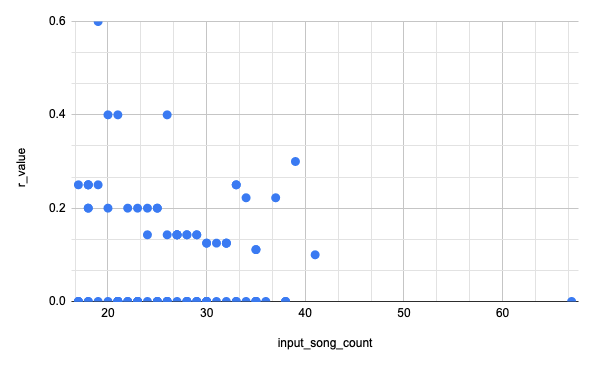
\includegraphics[scale=0.6]{images/80_big_sets}
	\centering
	\caption{Scatter graph of r-precision values with latent factors as 80 pulling from larger DJ sets} 
\end{figure}


\section{Comparing with industry-standard models}

The concept of calculating an R-precision value was introduced in the RecSys 2018 Spotify playlist dataset, where participants were tasked with building music recommendation systems for a given playlist. Normalised Discounted Cumulative Gain and Recommended Song Clicks were also used to measure the quality of the application. Figure 7.4 illustrates the highest-performing teams in the said convention. The maximum average value attained by the application in question was 0.1207, which is significantly lower compared to the top 10 values. The dataset and challenge set was eventually made open to the public, and compared to the results found on the leaderboard, the application would have ranked 46th. 

Its low ranking suggests the proposed method is unsuitable for finding valid recommendations for a given DJ set. This is due to the low average r-precision value when inputting a collection of DJ sets.
\begin{figure}[H]
	\hspace*{-0.5cm} 
	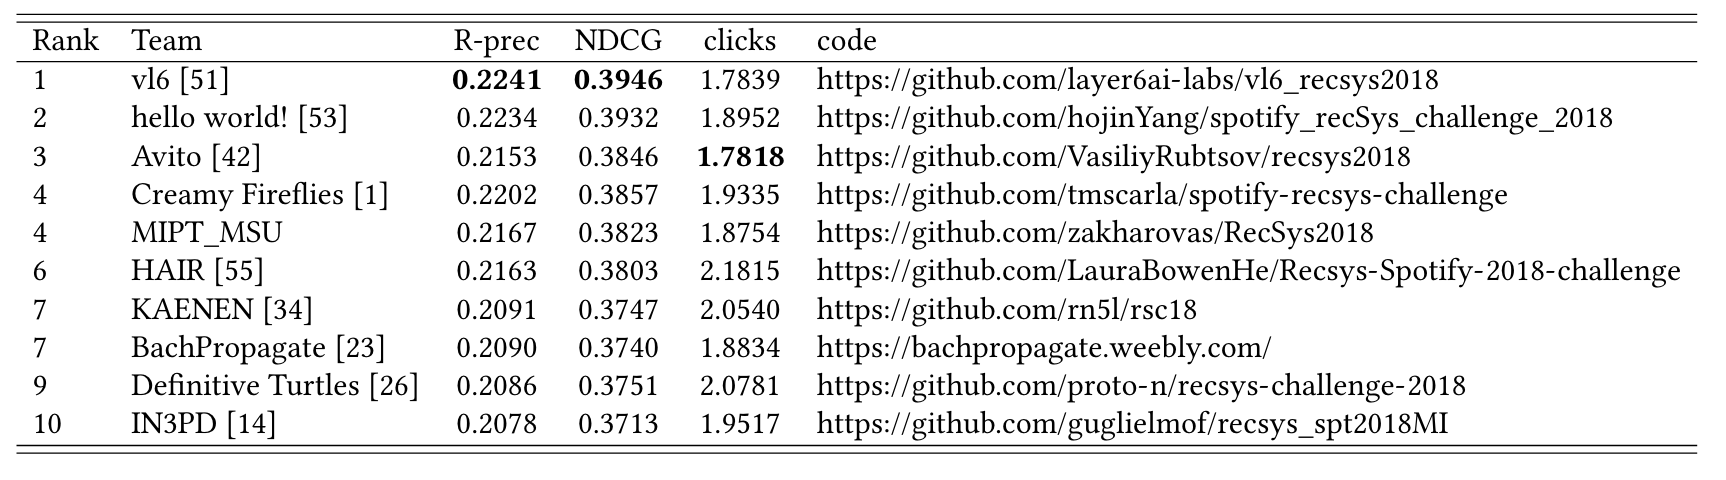
\includegraphics[scale=0.55]{images/recsys_scores}
	\caption{Top 10 Teams for RecSys 2018 and their given scores \citep{zamani_analysis_2019}} 
\end{figure}

\section{Summary}
Two experiments were conducted. The first was finding the highest average r-precision value by changing the latent factors used in the alternating least squares part of the model. After the latent factor value that obtained the highest r-precision value was found, the input song count of the DJ sets was changed. This did not improve the average r-precision value. The highest scoring average r-precision value was compared with the top performing models of the \textit{RecSys} 2018 convention. The proposed model scored considerably lower. 
% note that \Blindocument has 5 numbered levels, despite setting secnumdepth above. I (and many style guides) would suggest using no more than 3 numbered levels (incl. the chapter), with the option of a fourth unnumbered level.